% Created 2024-09-03 Tue 09:49
% Intended LaTeX compiler: pdflatex
\documentclass[aspectratio=169,xcolor={dvipsnames,svgnames}]{beamer}
\usepackage[utf8x]{inputenc}
\usepackage[T1]{fontenc}
\usepackage{graphicx}
\usepackage{longtable}
\usepackage{wrapfig}
\usepackage{rotating}
\usepackage[normalem]{ulem}
\usepackage{amsmath}
\usepackage{amssymb}
\usepackage{capt-of}
\usepackage{hyperref}
\usepackage{minted}
\usepackage{libertine}
\usepackage[normalem]{ulem}
\usepackage{varwidth}
\usepackage[Export]{adjustbox}
%\usepackage{enumitem}
\usepackage[linesnumbered,ruled,vlined]{algorithm2e}
\graphicspath{ {./careful-Isaac-Images/} {./org-download-images/} }
\usepackage[date=year,%
backend=biber,%
style=alphabetic,%
maxnames=5,%
minnames=3,%
maxalphanames=4,%
minalphanames=3,%
backref=true,%
doi=false,%
isbn=false,%
url=false,%
eprint=false]{biblatex}
\DefineBibliographyStrings{english}{%
backrefpage  = {\lowercase{s}ee p.}, % for single page number
backrefpages = {\lowercase{s}ee pp.} % for multiple page numbers
}
\addbibresource{/home/bvraghav/bibliography.bib}
%% Math typesetting
%% --------------------------------
\usepackage{amsmath}
\usepackage{amssymb}
\usepackage{amsfonts}
\usepackage{bbold}
% Operators with limit-style sub and superscript
\DeclareMathOperator*{\E}{\mathbb{E}}
\hypersetup{%
colorlinks=true,%
allcolors=magenta,%
%linkbordercolor = {white},%
%<your other options...>,
}
\usetheme{boxes}
\usecolortheme{crane}
\usefonttheme{serif}
\useinnertheme{rectangles}
\useoutertheme{}
\date{}
\title{mca101 : computer graphics}
\subtitle{color representation}
\author{%
%\noindent{} \\[2em]
\normalsize Raghav B. Venkataramaiyer
}
\institute{%
CSED TIET Patiala India.
}
\date{\scriptsize \today}
\setbeamercolor{alerted text}{fg=red!80!black}
%% Setup outline at begin section
%% -------------------------------------------------------
\AtBeginSection[]               % Section
{
\begin{frame}{outline}
\tableofcontents[currentsection,hideallsubsections]
\end{frame}
}
\AtBeginSubsection[]            % SubSection
{
\begin{frame}{outline}
\tableofcontents[currentsection,currentsubsection,subsectionstyle=show/shaded/hide]
\end{frame}
}
\setbeamerfont{structure}{shape=\scshape,family=\sffamily}
\setbeamertemplate{section page}
{
\begin{centering}
\begin{beamercolorbox}[sep=12pt,center]{part title}
\usebeamerfont{section title}\insertsection\par
\end{beamercolorbox}
\end{centering}
}

\setbeamercovered{transparent}
\hypersetup{
 pdfauthor={B.V. Raghav},
 pdftitle={mca101 : computer graphics},
 pdfkeywords={},
 pdfsubject={},
 pdfcreator={Emacs 29.4 (Org mode 9.6.24)}, 
 pdflang={English}}
\begin{document}

\maketitle

\section{colours --- introduction}
\label{sec:org92a7174}

\begin{frame}[label={sec:org215904e}]{what are colours}
\begin{columns}
\begin{column}{.5\columnwidth}
\begin{quote}
Colour is the \alert{visual perception} based on the
\alert{electromagnetic spectrum}. Though color is not an
\alert{inherent property} of matter, color perception is
related to an object's \alert{light absorption},
\alert{reflection}, \alert{emission spectra}, and \alert{interference}
--- \href{https://en.wikipedia.org/wiki/Color}{Wikipedia}
\end{quote}
\end{column}

\begin{column}{.5\columnwidth}
\begin{figure}[htbp]
\centering

\includegraphics[width=.9\linewidth]{images/Colouring_pencils.jpg}
\caption{Image Courtesy: \href{https://en.wikipedia.org/wiki/File:Colouring\_pencils.jpg}{Wikipedia}}
\end{figure}
\end{column}
\end{columns}
\end{frame}

\begin{frame}[label={sec:org868abc7}]{rgb colours}
\begin{columns}
\begin{column}{.5\columnwidth}
\begin{quote}
Perception of color originates from different light
wavelength or spectral sensitivity in cone cell types,
which is then processed by the brain.

For most humans, colors are perceived in the visible
light spectrum with three types of cone cells
(trichromacy)

--- \href{https://en.wikipedia.org/wiki/Color}{Wikipedia}
\end{quote}
\end{column}

\begin{column}{.5\columnwidth}
\begin{figure}[htbp]
\centering
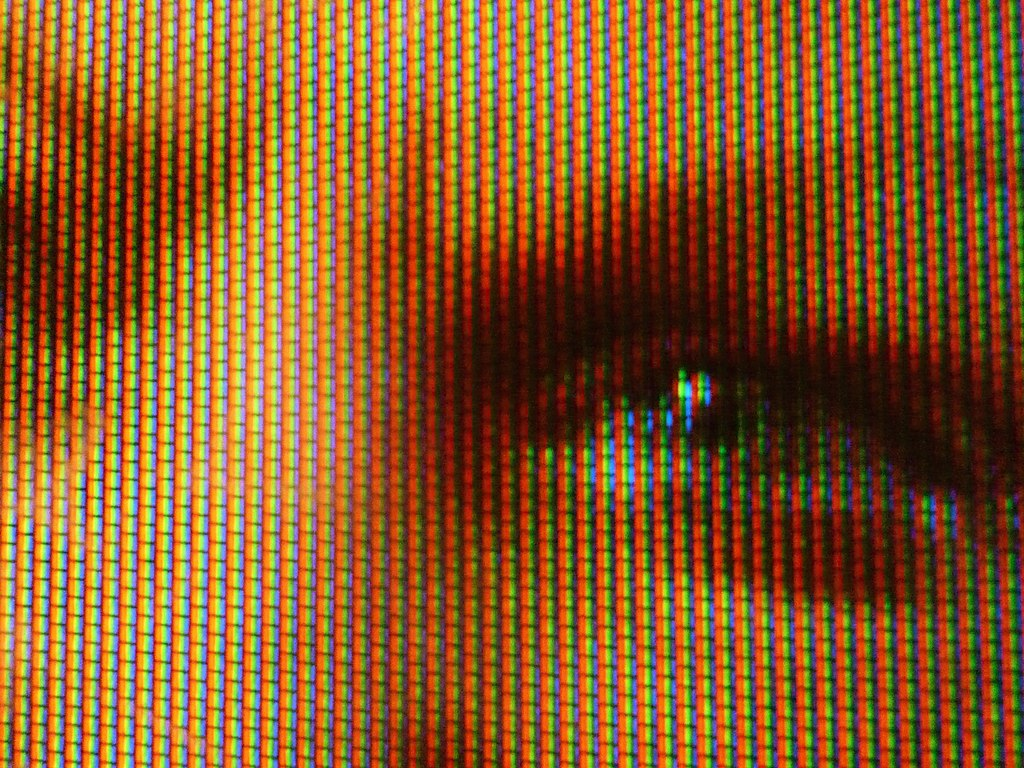
\includegraphics[width=.9\linewidth]{images/Tricolour_television_close_up.jpg}
\caption{Image Courtesy: \href{https://upload.wikimedia.org/wikipedia/commons/f/f9/Tricolour\_television\_close\_up.jpg}{Wikipedia}}
\end{figure}
\end{column}
\end{columns}
\end{frame}

\begin{frame}[label={sec:org0b372c8}]{visible spectrum}
\begin{figure}[htbp]
\centering
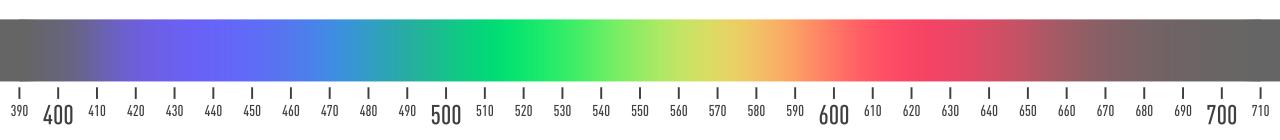
\includegraphics[width=.9\linewidth]{images/Visible_spectrum_390-710_nm_linear_perceptual.svg.png}
\caption{Visible Spectrum. Courtesy: \href{https://en.wikipedia.org/wiki/File:Visible\_spectrum\_390-710\_nm\_linear\_perceptual.svg}{Wikipedia}}
\end{figure}
\end{frame}

\begin{frame}[label={sec:orgcc24d32}]{rgb/a representation}
A colour in machine representation is
\begin{itemize}
\item a 3-vector for RGB,  i.e.
\begin{itemize}
\item \(\mathbf{c}\in\mathbb{R}_{[0,1]}^3\) in
floating-point representation;
\item \(\mathbf{c}\in\mathbb{Z}_{[0,255]}^3\) in 8-bit
fixed-point representation.
\end{itemize}
\item a 4-vector for RGBA,  i.e.
\begin{itemize}
\item \(\mathbf{c}\in\mathbb{R}_{[0,1]}^4\) in
floating-point representation;
\item \(\mathbf{c}\in\mathbb{Z}_{[0,255]}^4\) in 8-bit
fixed-point representation.
\end{itemize}
\end{itemize}
\end{frame}

\subsection{Image Representation}
\label{sec:orgb599fd4}

\begin{frame}[label={sec:org3a87706}]{an image as composition of pixels}
\begin{columns}
\begin{column}{.67\columnwidth}
\begin{itemize}
\item An \alert{image} is represented in \uline{pixels};
\item Conceptually, an image may be thought of split into a
\alert{rectangular grid} of height \(H\) and width \(W\);
\item Each cell of such a grid, is called a \alert{pixel}. A
pixel is the smallest unit of area patch in an image
and contains a uniform colour throughout;
\item \(H\times W\) is called \alert{the resolution} of such an
image.
\end{itemize}
\end{column}
\end{columns}
\end{frame}

\begin{frame}[label={sec:org70a4177}]{an image as a bounded space}
\begin{columns}
\begin{column}{.67\columnwidth}
\begin{itemize}
\item An optical camera sensor receives \alert{coloured signals}
within the spatial opening from its shutter;
\item The sensor registers the signals as energy/ intensity
corresponding to each of the R,G,B frequencies of
visible spectrum.
\item The signals are physically \alert{continuous} in space.
\item In practice, samples are \alert{discrete} in space.
\item The space is 2-dimensional and \alert{bound} on top, bottom,
left and right.
\item Hence an image may also be interpreted as \alert{a
quantised and bounded spatial signal}.
\end{itemize}
\end{column}
\end{columns}
\end{frame}


\begin{frame}[label={sec:orgfc55c46}]{image channels}
\begin{columns}
\begin{column}{.67\columnwidth}
\begin{itemize}
\item Each of R, G, B, A etc. are known as channels.
\item If a camera may sample more frequencies, including
ultra- and infra-optical spectrum, the resulting
image is called a hyper-spectral image.
\item The RGB image has 3-channels
\item The RGBA image has 4-channels
\item A hyper-spectral image may have many channels, say
\(C\) channels.
\end{itemize}
\end{column}
\end{columns}
\end{frame}

\begin{frame}[label={sec:org6e8d88d}]{image in floating-point representation}
\begin{columns}
\begin{column}{.67\columnwidth}
A floating-point may be 16-bit, 32-bit or 64-bit per
channel, generally used internally within graphic
frameworks like OpenGL/ WebGL etc.

\vspace{\baselineskip}

An image with resolution \(H\times W\), \\[0pt]
containing \(C\) channels \\[0pt]
is represented as
\(\mathbf{x}\in\mathbb{R}_{[0,1]}^{C\times H\times W}\).

\vspace{\baselineskip}

An RGB image with resolution \(H\times W\), \\[0pt]
is represented as \(\mathbf{x}\in\mathbb{R}_{[0,1]}^{3\times
H\times W}\).

\vspace{\baselineskip}

An RGBA image with resolution \(H\times W\), \\[0pt]
is represented as \(\mathbf{x}\in\mathbb{R}_{[0,1]}^{4\times
H\times W}\).
\end{column}
\end{columns}
\end{frame}

\begin{frame}[label={sec:orgde60624}]{image in 8-bit fixed-point}
\begin{columns}
\begin{column}{.67\columnwidth}
A fixed-point may be 8-bit, 16-bit, 32-bit or 64-bit
per channel, generally 8-bit is most commonly used.

\vspace{\baselineskip}

An image with resolution \(H\times W\), \\[0pt]
containing \(C\) channels \\[0pt]
is represented as \(\mathbf{x}\in\mathbb{Z}_{[0,255]}^{C\times
H\times W}\).

\vspace{\baselineskip}

An RGB image with resolution \(H\times W\), \\[0pt]
is represented as \(\mathbf{x}\in\mathbb{Z}_{[0,255]}^{3\times
H\times W}\).

\vspace{\baselineskip}

An RGBA image with resolution \(H\times W\), \\[0pt]
is represented as
\(\mathbf{x}\in\mathbb{Z}_{[0,255]}^{4\times H\times W}\).
\end{column}
\end{columns}
\end{frame}

\begin{frame}[label={sec:orgfd159c2}]{question}
\begin{enumerate}
\item How is a grayscale image with resolution \(H\times W\)
with floating-point representation described
mathematically?
\item How is a grayscale image with resolution \(H\times W\)
with 8-bit fixed-point representation described
mathematically?
\item How is a grayscale image with resolution \(H\times W\)
with 16-bit fixed-point representation described
mathematically?
\end{enumerate}
\end{frame}

\begin{frame}[label={sec:orgf57e3cd}]{question}
\begin{enumerate}
\item What is the minimum size (in bytes) required to store an
uncompressed RGB image in FHD resolution. Assume the
image header to be \(H\) bytes.
\item What is the minimum size (in bytes) required to
store an uncompressed RGBA image in FHD
resolution. Assume the image header to be \(H\) bytes.
\end{enumerate}
\end{frame}

\section{colour tables}
\label{sec:org315a89c}

\begin{frame}[label={sec:orgd179344}]{colour tables}
\begin{columns}
\begin{column}{.67\columnwidth}
In order to improve storage efficiency of images,

\vspace{\baselineskip}
\begin{itemize}
\item Included colours are listed, the count \(n<256\)
generally.  This is called a colour table.
\item For each pixel, the colour is approximated and
assigned to be one of the colours in the table, and
the colour index is stored instead of the complete
colour information.
\item This reduces the storage requirement by order of
magnitude.
\item The only additional storage requirement is that of
the colour table, \(n\times3\) bytes
\end{itemize}
\end{column}
\end{columns}
\end{frame}
\begin{frame}[label={sec:orgd74e1eb}]{storage efficiency}
\begin{columns}
\begin{column}{.67\columnwidth}
For example,
\begin{itemize}
\item RGB image requires \(8\times3 = 24\) bits per pixel;
whereas
\item Colour table with upto 2 colours would require only
1-bit per pixel;
\item Colour table with 3-4 colours would require only
2-bit per pixel;
\item Colour table with 5-8 colours would require only
3-bit per pixel;
\end{itemize}
\end{column}
\end{columns}
\end{frame}
\begin{frame}[label={sec:org4833691}]{storage efficiency}
\begin{columns}
\begin{column}{.67\columnwidth}
\begin{center}
\begin{tabular}{rr}
Num Bits & Max Num Colours\\[0pt]
\hline
1 & 2\\[0pt]
2 & 4\\[0pt]
3 & 8\\[0pt]
4 & 16\\[0pt]
5 & 32\\[0pt]
6 & 64\\[0pt]
7 & 128\\[0pt]
8 & 256\\[0pt]
\end{tabular}
\end{center}
\end{column}
\end{columns}
\end{frame}


\begin{frame}[label={sec:org9de940d}]{question}
\begin{columns}
\begin{column}{.67\columnwidth}
What is the minimum size (in bytes) of storage required
to store an image with colour table with 100
RGB-colours? Assume the image header to be \(H\) bytes.
\end{column}
\end{columns}
\end{frame}

\section{colour spaces}
\label{sec:org04ded5b}

\begin{frame}[label={sec:org3c6f465}]{hsl and hsv}
\begin{columns}
\begin{column}{.4\columnwidth}
\begin{figure}[htbp]
\centering
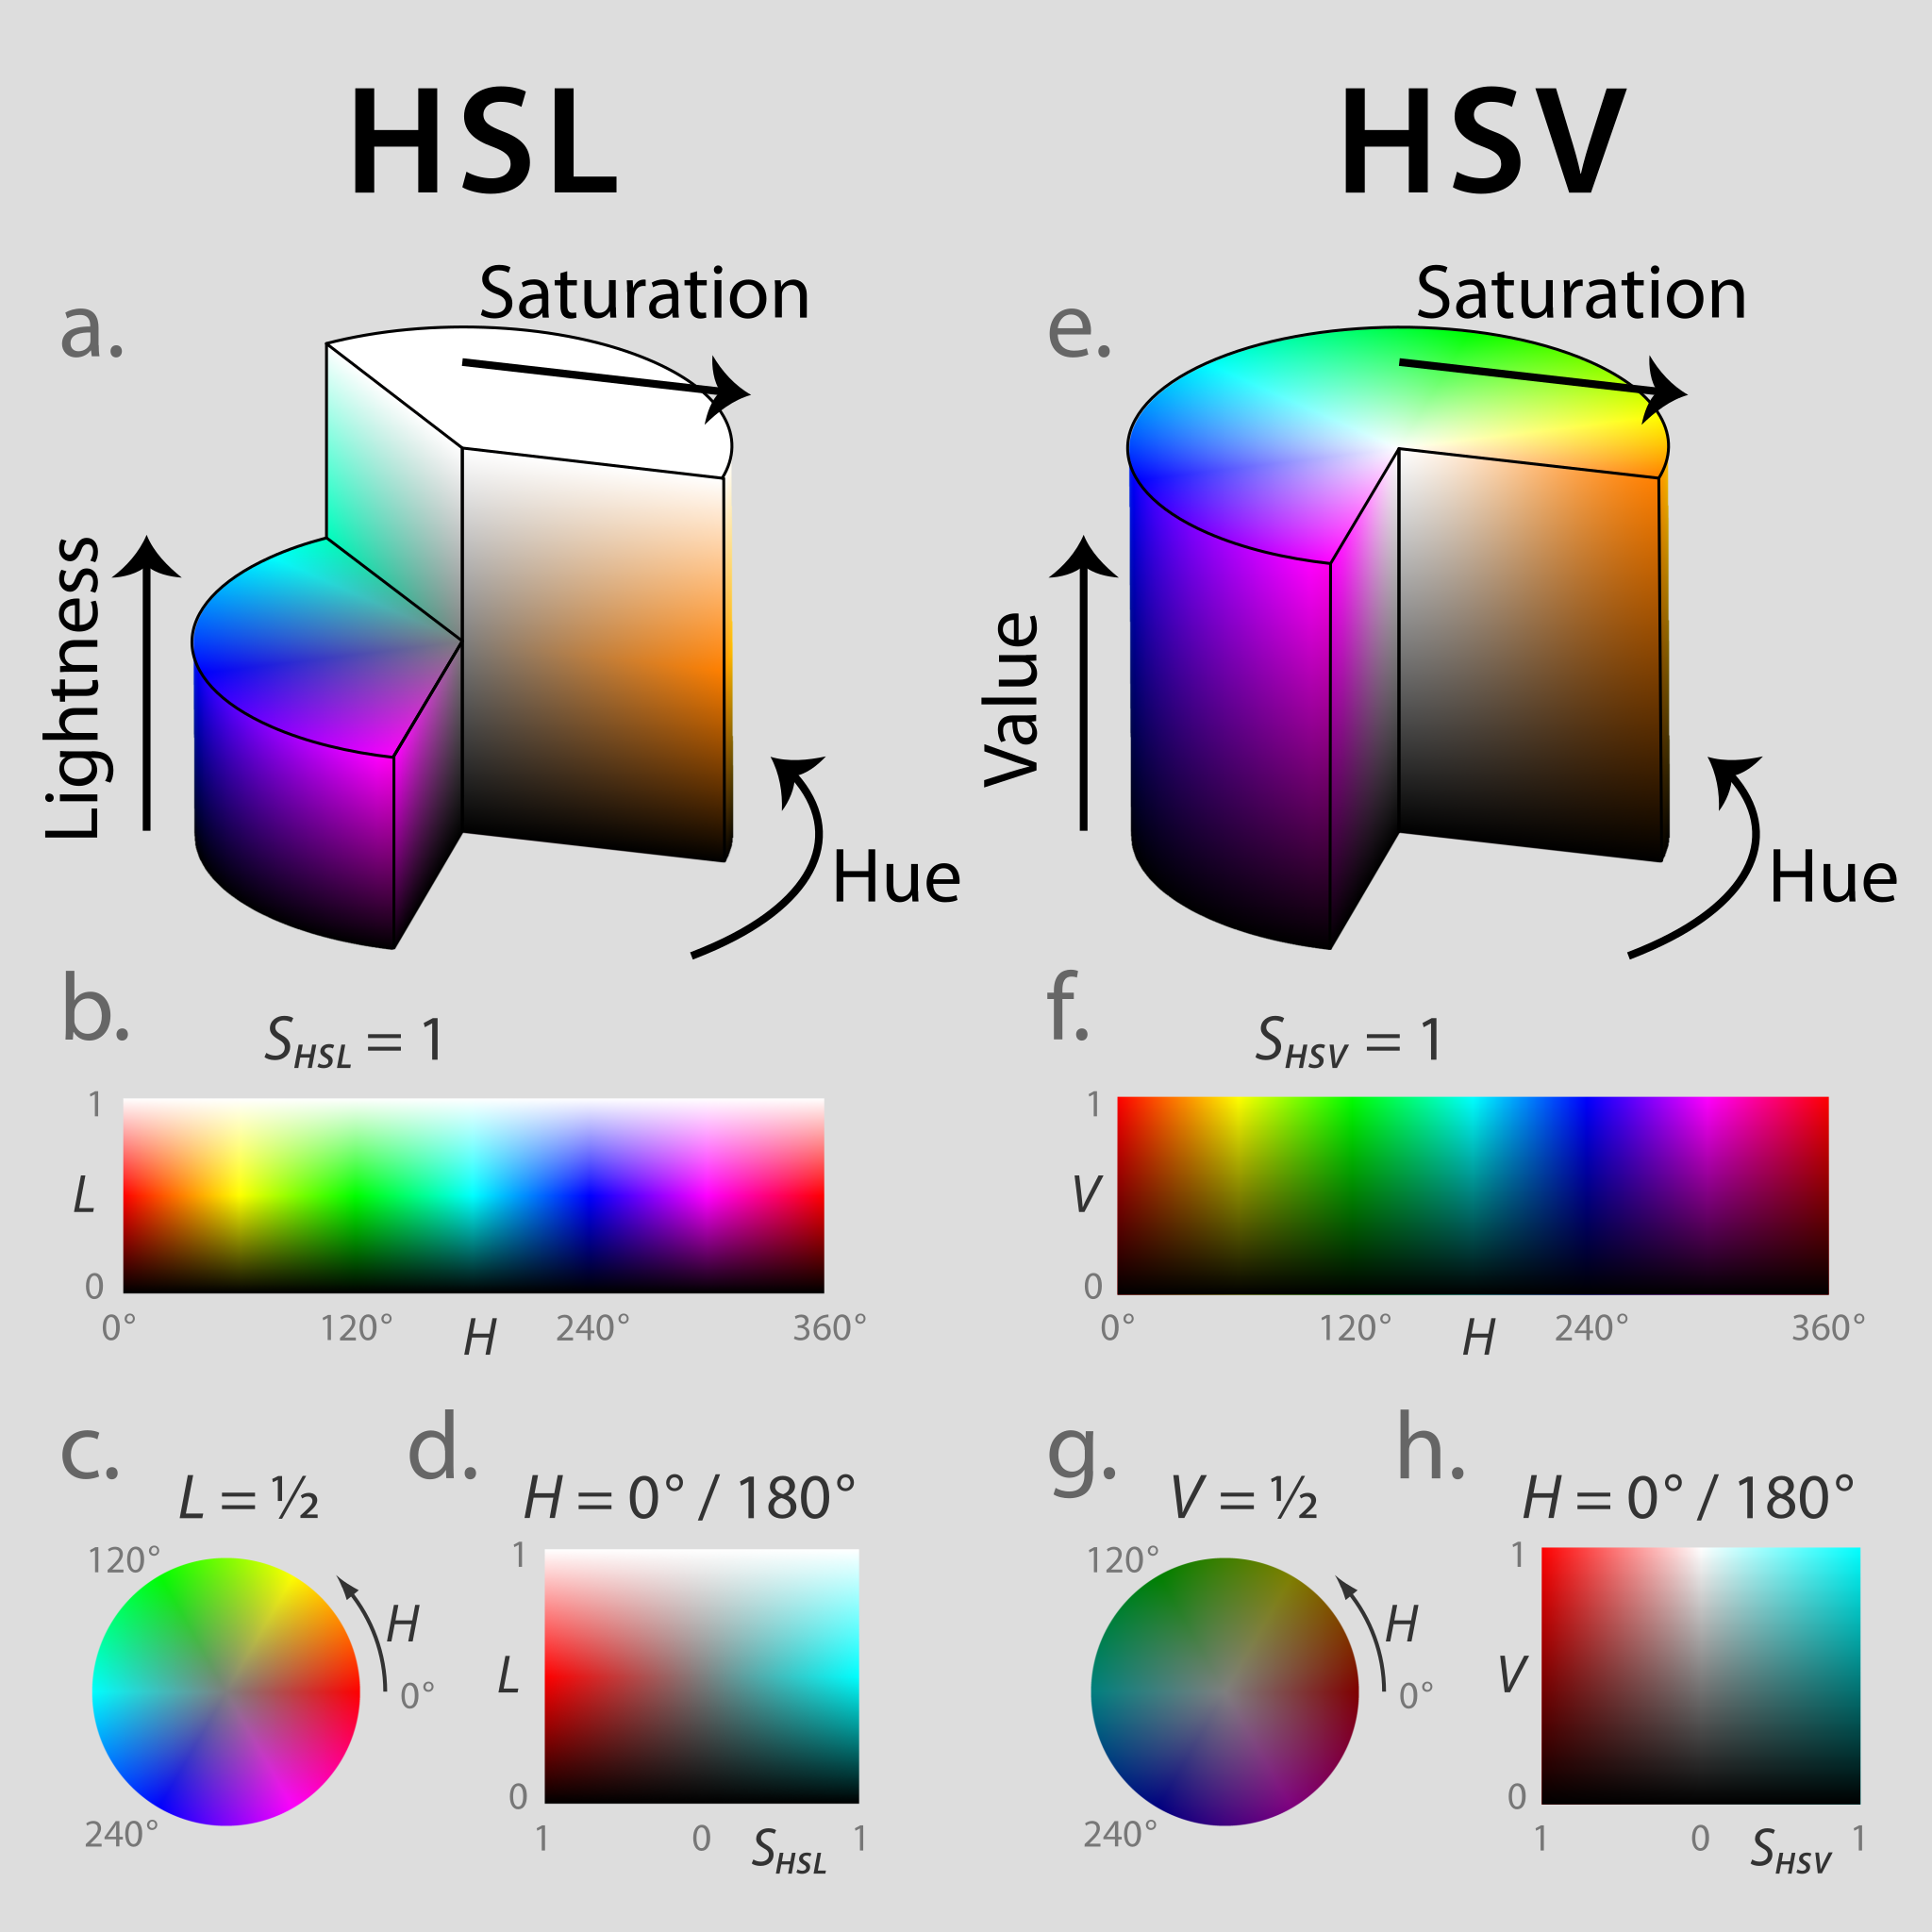
\includegraphics[width=.9\linewidth]{images/Hsl-hsv_models.svg.png}
\caption{Image Courtesy: \href{https://commons.wikimedia.org/wiki/File:Hsl-hsv\_models.svg}{Wikipedia}}
\end{figure}
\end{column}
\end{columns}
\end{frame}

\begin{frame}[label={sec:org78cc9f3}]{cmyk (print technology)}
\begin{columns}
\begin{column}{.5\columnwidth}
\begin{figure}[htbp]
\centering

\includegraphics[width=0.65\linewidth]{images/CMYK_color_model.svg.png}
\caption{When subtractive CMY inks are combined at full strength, pairwise combinations are red, green, and blue. Combining all three gives an imperfect black colour.}
\end{figure}
\end{column}

\begin{column}{.5\columnwidth}
\begin{figure}[htbp]
\centering

\includegraphics[width=0.65\linewidth]{images/CMYK_Color_Swatches.svg.png}
\caption{Color printing typically uses ink of four colours: cyan, magenta, yellow, and black.}
\end{figure}
\end{column}
\end{columns}
\end{frame}

\begin{frame}[label={sec:org18a3fdb}]{rgb vs cmyk}
\begin{columns}
\begin{column}{.5\columnwidth}
\begin{center}
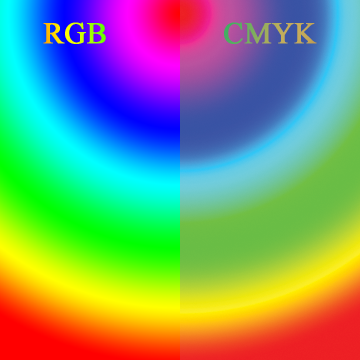
\includegraphics[width=.9\linewidth]{images/RGB_and_CMYK_comparison.png}
\end{center}
\end{column}

\begin{column}{.5\columnwidth}
A comparison of CMYK and RGB color models. This image
demonstrates the difference between how colors will
look on a computer monitor (RGB) compared to how they
might reproduce in a particular CMYK print process.

\vspace{\baselineskip}

Image Courtesy: \href{https://commons.wikimedia.org/wiki/File:RGB\_and\_CMYK\_comparison.png}{Wikipedia}
\end{column}
\end{columns}
\end{frame}

\begin{frame}[label={sec:org98e45e0}]{colour mixing: additive vs subtractive}
\begin{columns}
\begin{column}{.5\columnwidth}
\textsc{additive colour mixing} \\[0pt]
Three overlapping light bulbs in a vacuum, adding
together to create white.

\begin{figure}[htbp]
\centering
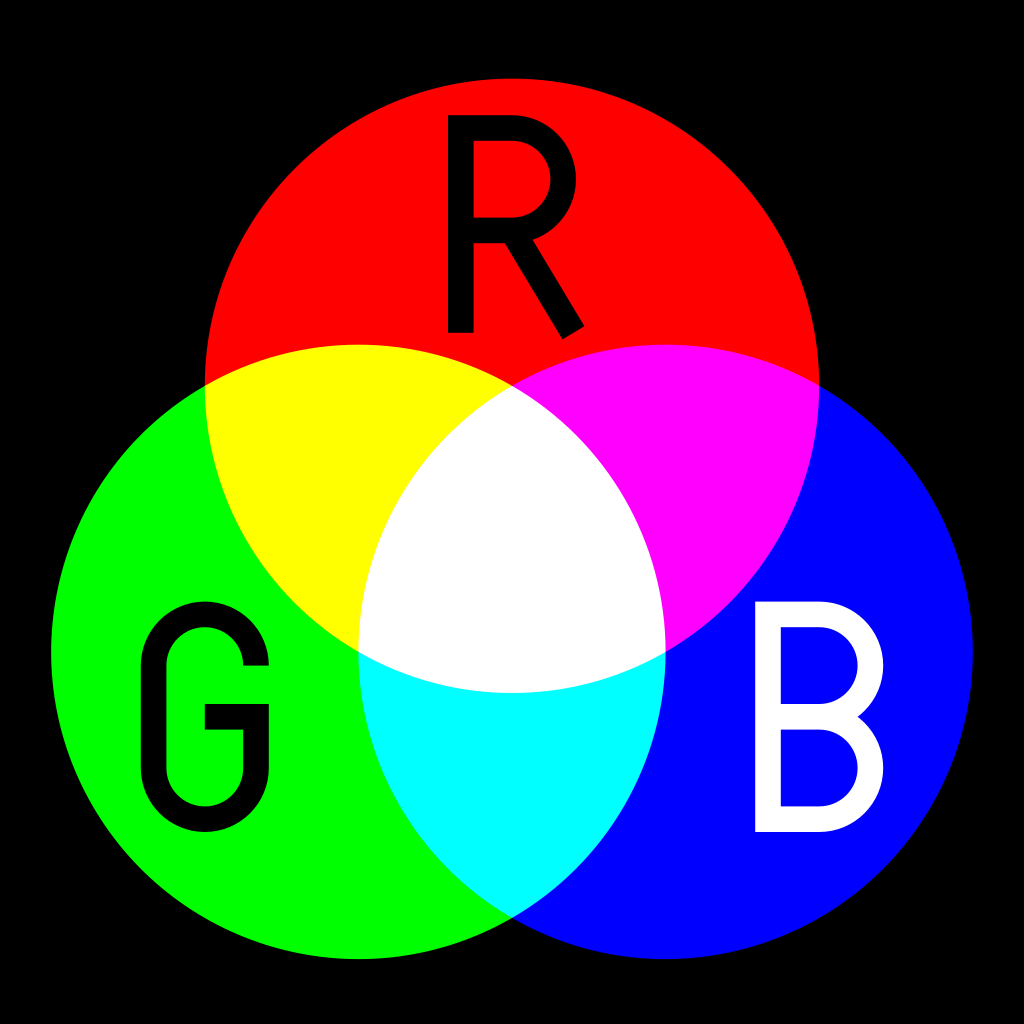
\includegraphics[width=0.6\linewidth]{images/AdditiveColor.svg.png}
\caption{Image Courtesy: \href{https://en.wikipedia.org/wiki/File:AdditiveColor.svg}{Wikipedia}}
\end{figure}
\end{column}
\begin{column}{.5\columnwidth}
\textsc{subtractive colour mixing} \\[0pt]
Three splotches of paint on white paper, subtracting
together to turn the paper black.

\begin{figure}[htbp]
\centering

\includegraphics[width=0.6\linewidth]{images/SubtractiveColor.svg.png}
\caption{Image Courtesy: \href{https://en.wikipedia.org/wiki/File:SubtractiveColor.svg}{Wikipedia}}
\end{figure}
\end{column}
\end{columns}
\end{frame}

\begin{frame}[label={sec:org0f96d8a}]{other colour spaces}
\begin{enumerate}
\item Munsell (Munsell Colour System)
\item Pantone (Pantone Matching System)
\item Colour Fan Decks (by Paint Manufacturers)
\item Y,u,v Colour Space
\item L,a,b Colour Space
\end{enumerate}


\href{https://en.wikipedia.org/wiki/List\_of\_color\_spaces\_and\_their\_uses}{(Read More)}
\end{frame}

\section{Interpolation}
\label{sec:orgbfc2d4f}

\subsection{Linear Interpolation}
\label{sec:orgea2efd0}

\begin{frame}[label={sec:org27fb44d}]{linear interpolation}
\begin{columns}
\begin{column}{.5\columnwidth}
Point on straight line segment connecting vectors
\(\mathbf{a},\mathbf{b}\), may be given parameterised by
\(t\in\mathbb{R}_{[0,1]}\) as,
\begin{align}
  \notag
  f(t) &= (1-t)\mathbf{a} + t\,\mathbf{b} \\
  \notag
  &= \mathbf{a} + t(\mathbf{b}-\mathbf{a})
\end{align}

\begin{align}
  \notag
  t=0 &\iff f(t) = \mathbf{a} \\
  \notag
  t=1 &\iff f(t) = \mathbf{b}
\end{align}
\end{column}
\end{columns}
\end{frame}


\begin{frame}[label={sec:orgafb95cd}]{linear interpolation}
\begin{columns}
\begin{column}{.3\columnwidth}
\alert{Question} \\[0pt]
Given two points \(\mathbf{a},\mathbf{b} \in
\mathbb{R}^2\), find the point on straight line
connecting them, and in between, so that it is twice as
far away from \(\mathbf{b}\) as it is from \(\mathbf{a}\).
\end{column}

\begin{column}{.7\columnwidth}
\alert{Solution} \\[0pt]
Point on straight line connecting
\(\mathbf{a},\mathbf{b}\), and in between, may be given
parameterised by \(t\in\mathbb{R}_{[0,1]}\) as,
\begin{align}
  \notag
  f(t) = (1-t)\mathbf{a} + t\,\mathbf{b}
\end{align}

Here if the Euclidean distance \(\Delta_E (\mathbf{a},
\mathbf{b}) = 1\,\mathrm{unit}\), then \(\Delta_E
(\mathbf{a}, f(t)) = 1-t\,\mathrm{units}\), and
\(\Delta_E (f(t), \mathbf{b}) = t\,\mathrm{units}\).

Hence,
\begin{align}
  \notag
  t &= \frac23 \qquad \because t = 2(1-t) \\
  \notag
  \mathbf{p} &= f(t=\frac23) =
               \frac13\mathbf{a} + \frac23\mathbf{b}
\end{align}
\end{column}
\end{columns}
\end{frame}



\begin{frame}[label={sec:org766f1d9}]{linear interpolation}
\begin{columns}
\begin{column}{.3\columnwidth}
\alert{Question} \\[0pt]
Given two RGB colours \(\mathbf{a},\mathbf{b} \in
\mathbb{R}^3\), find the colour \(\mathbf{c}\), so that it
is twice as far away from \(\mathbf{b}\) as it is from
\(\mathbf{a}\).
\end{column}

\begin{column}{.7\columnwidth}
\alert{Solution} \\[0pt]
Point on hypothetical straight line in RGB colour space
connecting \(\mathbf{a},\mathbf{b}\), and in between, may
be given parameterised by \(t\in\mathbb{R}_{[0,1]}\) as,
\begin{align}
  \notag
  f(t) = (1-t)\mathbf{a} + t\,\mathbf{b}
\end{align}

Here if the Euclidean distance \(\Delta_E (\mathbf{a},
\mathbf{b}) = 1\,\mathrm{unit}\), then \(\Delta_E
(\mathbf{a}, f(t)) = 1-t\,\mathrm{units}\), and
\(\Delta_E (f(t), \mathbf{b}) = t\,\mathrm{units}\).

Hence,
\begin{align}
  \notag
  t &= \frac23 \qquad \because t = 2(1-t) \\
  \notag
  \mathbf{p} &= f(t=\frac23) =
               \frac13\mathbf{a} + \frac23\mathbf{b}
\end{align}
\end{column}
\end{columns}
\end{frame}





\subsection{Barycentric Interpolation}
\label{sec:org4aaf7e3}

\begin{frame}[label={sec:org2fb5744}]{barycentric coordinates}
\begin{columns}
\begin{column}{.3\columnwidth}
\begin{figure}[htbp]
\centering
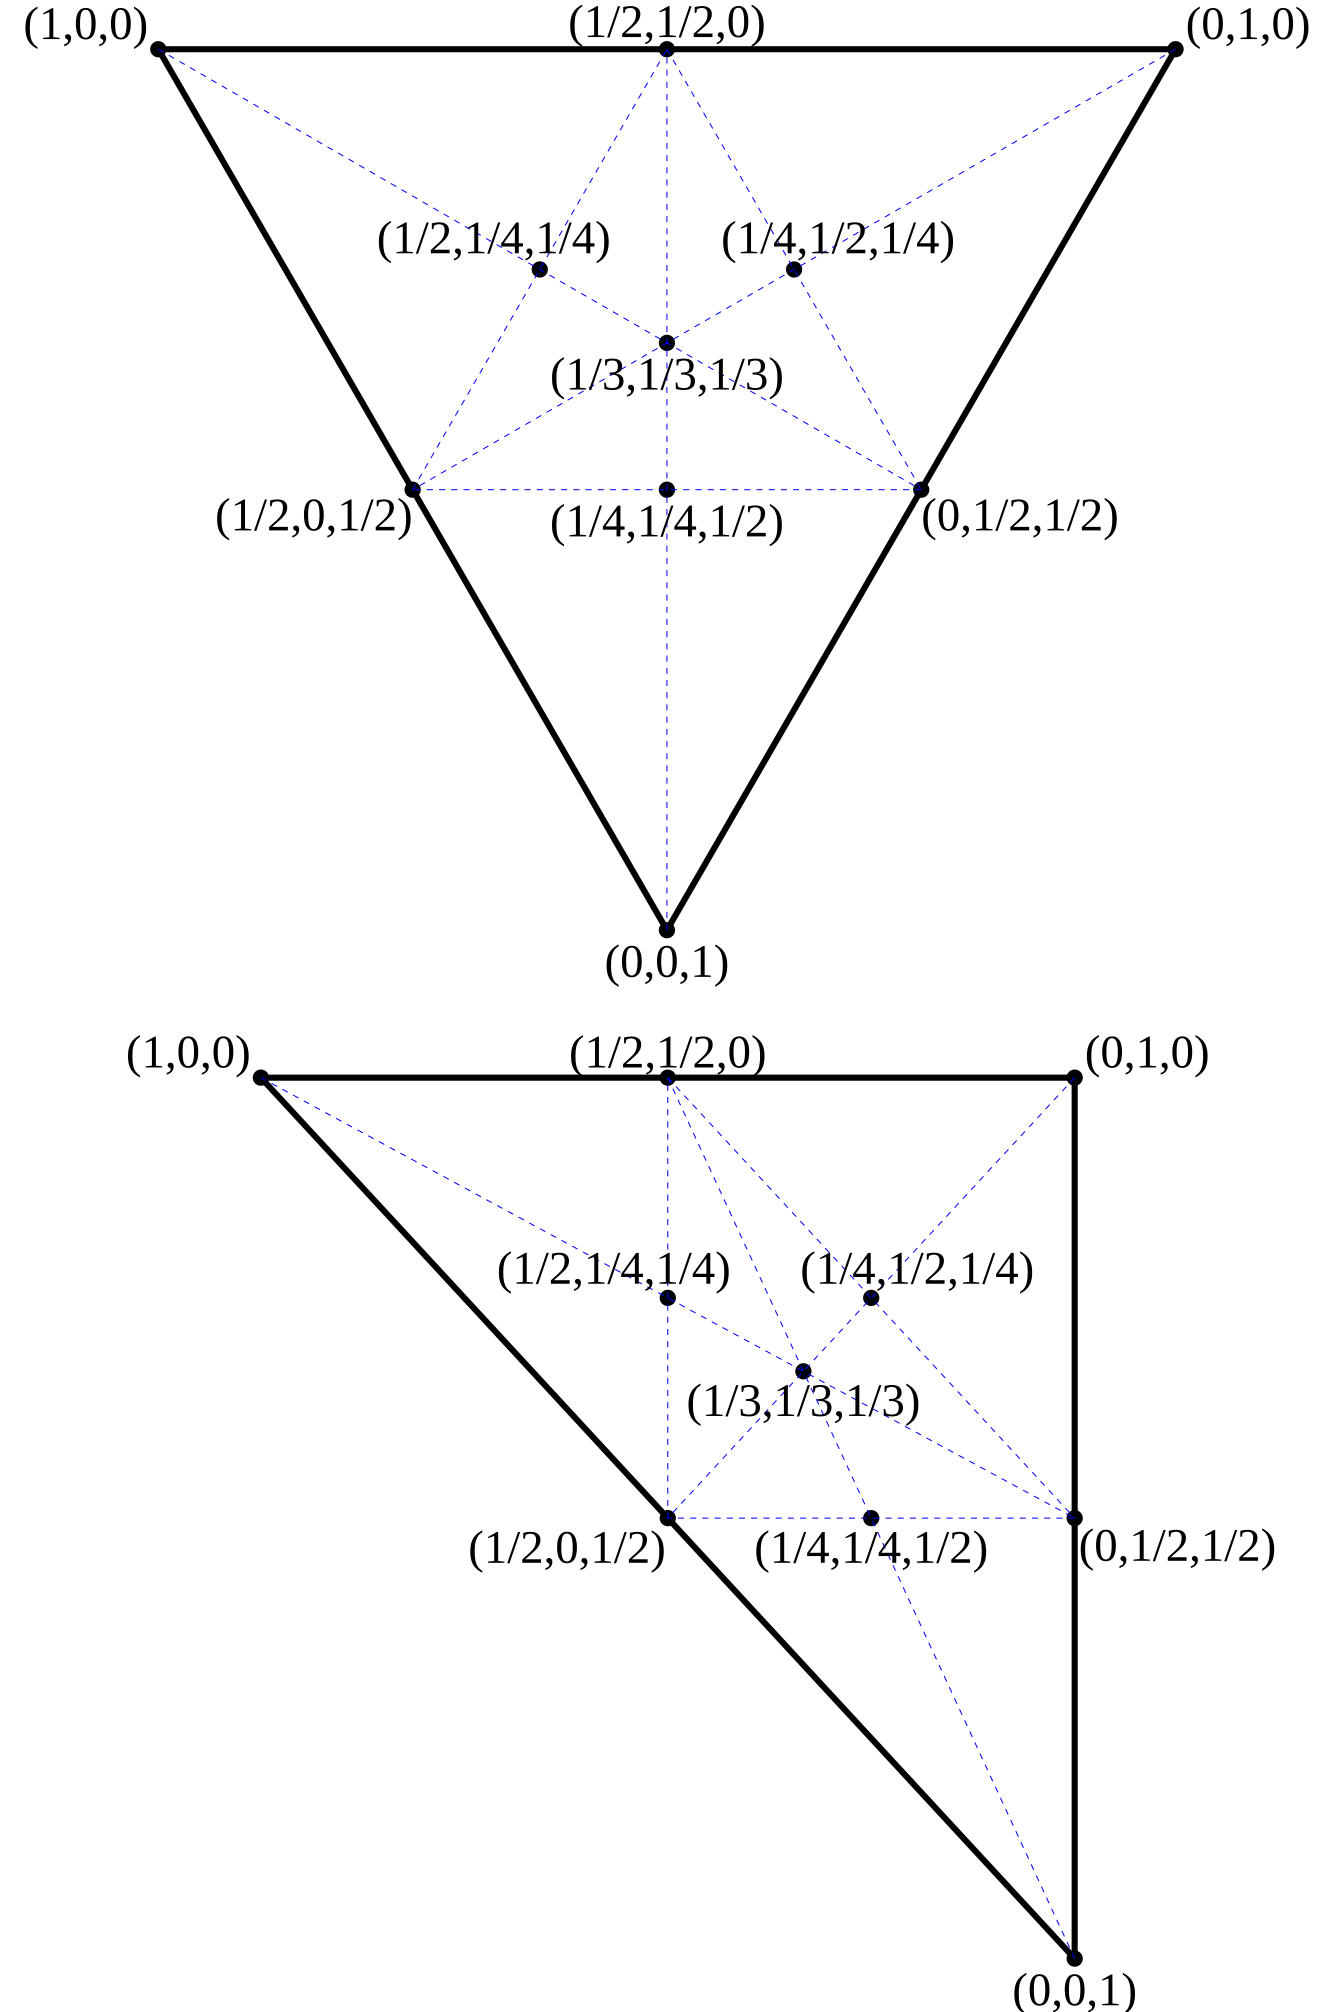
\includegraphics[width=.9\linewidth]{images/TriangleBarycentricCoordinates.svg.png}
\caption{Image Courtesy: \href{https://commons.wikimedia.org/wiki/File:TriangleBarycentricCoordinates.svg}{Wikipedia}}
\end{figure}
\end{column}

\begin{column}{.5\columnwidth}
With respect to the vertices \(\mathbf{a}\), \(\mathbf{b}\)
and \(\mathbf{c}\), the points inside the triangle may be
represented as \((\lambda_{a},\lambda_{b},\lambda_{c})\),
where \(\lambda_{a} + \lambda_{b} + \lambda_{c} = 1\).
\end{column}
\end{columns}
\end{frame}

\begin{frame}[label={sec:org0c3ab12}]{barycentric coordinates}
\begin{columns}
\begin{column}{.3\columnwidth}
\begin{figure}[htbp]
\centering
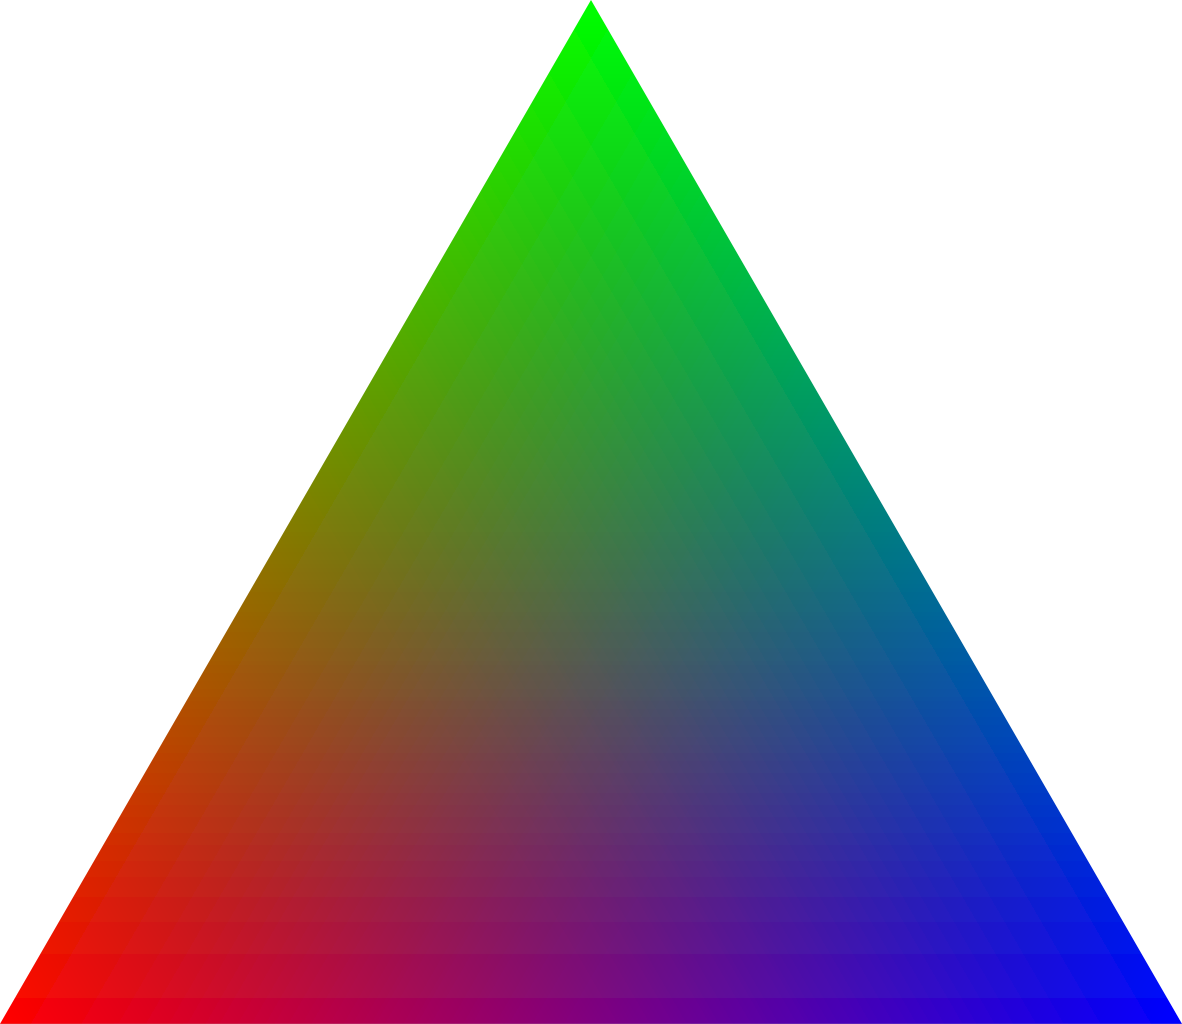
\includegraphics[width=.9\linewidth]{images/Barycentric_RGB.svg.png}
\caption{Barycentric coordinates are used for blending three colors over a triangular region evenly in computer graphics. Image Courtesy: \href{https://commons.wikimedia.org/wiki/File:Barycentric\_RGB.svg}{Wikipedia}}
\end{figure}
\end{column}

\begin{column}{.5\columnwidth}
With respect to the vertices \(\mathbf{a}\), \(\mathbf{b}\)
and \(\mathbf{c}\), the points inside the triangle may be
represented as \((\lambda_{a},\lambda_{b},\lambda_{c})\),
where \(\lambda_{a} + \lambda_{b} + \lambda_{c} = 1\).
\end{column}
\end{columns}
\end{frame}
\end{document}
